%! alt A convex 10-gon divided into triangles by 7 non-crossing diagonals. The shaded triangle has two polygon sides, va and vb, so no diagonal leaves v and the third side ab is a drawn diagonal. Removing v leaves a triangulated 9-gon in which ab is a side.
%! after_paragraph 3
%! scale 3/100
% The shared preamble of every Kyuclid figure. pipeline/figures turns these colours into theme-aware paint,
% and refuses any other colour, so draw only with them:
%   figink (lines and labels), figaux (construction lines), figaccent (the object the argument turns on),
%   figtint and figaccenttint (light fills).
\documentclass[border=1.5pt]{standalone}
\usepackage{tkz-euclide}
\definecolor{figink}{RGB}{0,0,0}
\definecolor{figaux}{RGB}{85,85,85}
\definecolor{figaccent}{RGB}{192,57,43}
\definecolor{figtint}{RGB}{221,221,221}
\definecolor{figaccenttint}{RGB}{245,213,208}
% tkz-euclide's defaults draw circles, compasses and marks in 50% grey and fill points with a tint.
\makeatletter
\def\tkz@otherlinecolor{figink}
\def\tkz@euc@circlecolor{figink}
\def\tkz@euc@compasscolor{figink}
\def\tkz@euc@mkcolor{figink}
\def\tkz@mk@fill{figink}
\def\tkz@euc@pointfillcolor{figink}
\makeatother
\tkzSetUpLine[color=figink,line width=.7pt]
\tkzSetUpArc[color=figink,line width=.7pt]
\tkzSetUpCompass[color=figink,line width=.5pt]
\tkzSetUpPoint[color=figink,fill=figink,size=3.1pt]
\tikzset{
  every picture/.style={line cap=round,line join=round,color=figink},
  circle style/.append style={color=figink,line width=.7pt},
  aux/.style={color=figaux,line width=.45pt,dash pattern=on 2.6pt off 2pt},
  key/.style={color=figaccent,line width=1pt},
  mk/.style={color=figink,line width=.5pt},
  lbl/.style={color=figink,inner sep=2.2pt},
  len/.style={color=figink,inner sep=1.5pt,font=\small},
}

\begin{document}
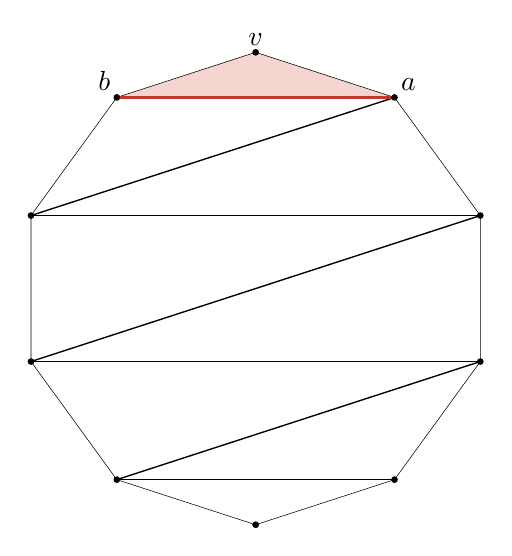
\begin{tikzpicture}
\tkzDefPoint(0.0,0.0){O} %! O = (0, 0)
\tkzDefPoint(0.0000000000000000000000000000000000000000000000000065022505,3.0000000){v} %! v = polar(O, 100, 90)
\tkzDefPoint(1.7633558,2.4270510){a} %! a = polar(O, 100, 54)
\tkzDefPoint(2.8531695,0.92705098){V2} %! V2 = polar(O, 100, 18)
\tkzDefPoint(2.8531695,-0.92705098){V3} %! V3 = polar(O, 100, -18)
\tkzDefPoint(1.7633558,-2.4270510){V4} %! V4 = polar(O, 100, -54)
\tkzDefPoint(0.0000000000000000000000000000000000000000000000000065022505,-3.0000000){V5} %! V5 = polar(O, 100, -90)
\tkzDefPoint(-1.7633558,-2.4270510){V6} %! V6 = polar(O, 100, -126)
\tkzDefPoint(-2.8531695,-0.92705098){V7} %! V7 = polar(O, 100, -162)
\tkzDefPoint(-2.8531695,0.92705098){V8} %! V8 = polar(O, 100, 162)
\tkzDefPoint(-1.7633558,2.4270510){b} %! b = polar(O, 100, 126)
%! fact equal(dist(v, a), dist(v, b))
%! fact equal(dist(V2, V3), dist(v, a))
%! fact concyclic(v, a, b, V4, V5, V6)
%! fact angle(a, v, b) == 144
\tkzFillPolygon[color=figaccenttint](v,a,b)
\tkzDrawPolygon(v,a,V2,V3,V4,V5,V6,V7,V8,b)
\tkzDrawSegments[line width=.5pt](a,V8 V2,V8 V2,V7 V3,V7 V3,V6 V4,V6)
\tkzDrawSegment[key](a,b)
\tkzDrawPoints(v,a,V2,V3,V4,V5,V6,V7,V8,b)
\tkzLabelPoint[above,lbl](v){$v$}
\tkzLabelPoint[above right,lbl](a){$a$}
\tkzLabelPoint[above left,lbl](b){$b$}
\end{tikzpicture}
\end{document}
